\documentclass[a5paper,twoside,12pt]{report}

%%%%%%%%%% Packages %%%%%%%%%%
\usepackage[outer=2cm, inner=2cm]{geometry}
\usepackage{hiero}
\usepackage{egypto}
\usepackage[backend=biber, style=authoryear-icomp]{biblatex}
\usepackage{fancyhdr}
\usepackage{microtype}
\usepackage{graphicx}
\usepackage{wrapfig}
\usepackage{enumitem}
\usepackage{amsmath}
\usepackage[utf8]{inputenc}
\usepackage[greek,english]{babel} 
\usepackage{epigraph}
\usepackage{lmodern}
\usepackage{afterpage}
\usepackage{nonumonpart}
\usepackage{titlesec}
\usepackage{microtype}
\usepackage{titling} 
\usepackage[T1]{fontenc}
\usepackage{bold-extra}
\usepackage{listings}
\usepackage{xcolor}
% \usepackage{draftwatermark}
\makeindex

\addbibresource{bibliography.bib}
\TextHieroglyphs

% \SetWatermarkText{Preview}
\newlength\longest
\setlength{\marginparwidth}{0pt}
\setlength{\headheight}{15pt}

\titleformat{\section}[wrap]
{\normalfont\bfseries}
{\thesection.}{0.5em}{}
\titlespacing{\section}{12pc}{1.5ex plus .1ex minus .2ex}{1pc}

\definecolor{backcolor}{rgb}{0.95,0.95,0.92}

\lstdefinestyle{mystyle}{
      backgroundcolor=\color{backcolor},
      basicstyle=\ttfamily\footnotesize,
      breakatwhitespace=false,         
      breaklines=true,                 
      captionpos=b,                    
      keepspaces=true,                 
      numbers=left,                    
      numbersep=5pt,                  
      showspaces=false,                
      showstringspaces=false,
      showtabs=false,                  
      tabsize=2
}
\lstset{style=mystyle}
%%%%%%%%%% Fancy HDR %%%%%%%%%%
\pagestyle{fancy}
\fancyhf{}
\fancyhead[LE,RO]{\thepage}
\fancyhead[LO]{\nouppercase{\leftmark}}
\fancyhead[RE]{\textsc{The Intricacies of Ancient Egyptian Hieroglyphics}}
\fancypagestyle{plain}{
\fancyhf{} 
\fancyhead[LE,RO]{\thepage}
\fancyhead[LO]{\leftmark}
\fancyhead[RE]{\textsc{The Intricacies of Ancient Egyptian Hieroglyphics}}}

\begin{document}
\pagenumbering{gobble} 

%%%%%%%%%% Pretitle %%%%%%%%%%
\thispagestyle{empty}
\begin{center}
	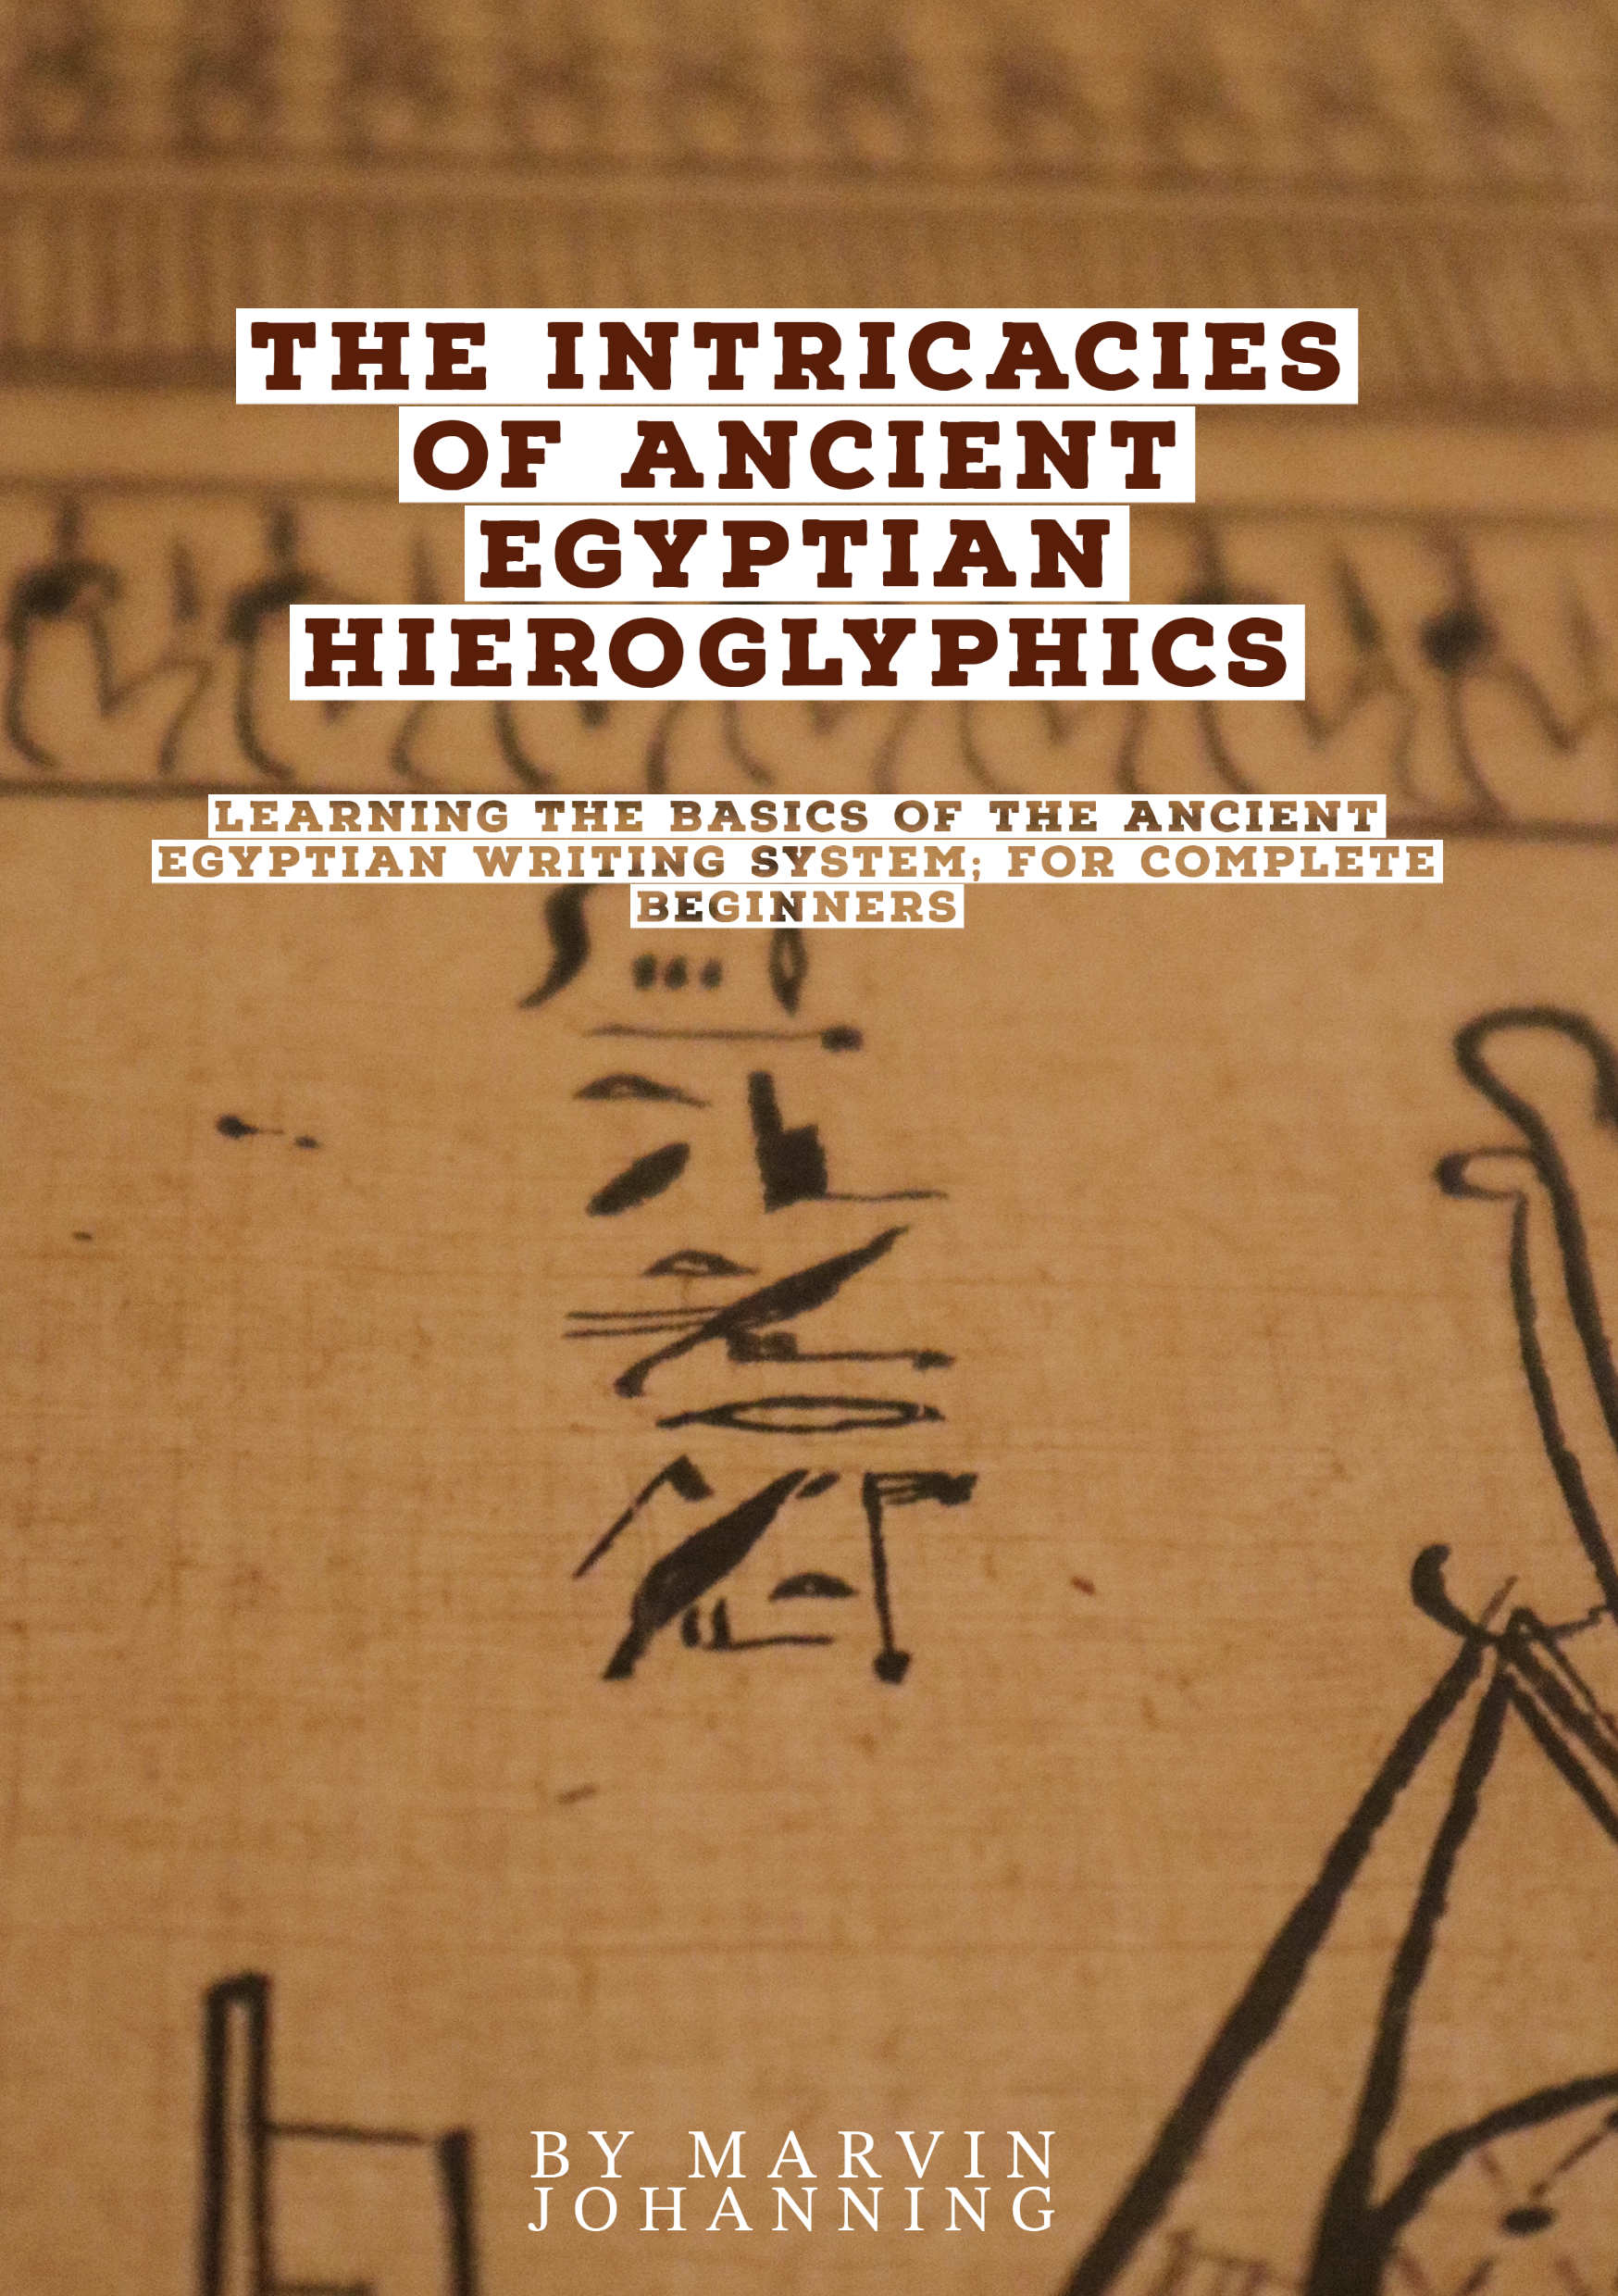
\includegraphics[scale=0.162]{cover.png}
\end{center}
\newpage

%%%%%%%%%% EMPTY PAGE %%%%%%%%%% 
\thispagestyle{empty}
  \mbox{}
  \newpage

%%%%%%%%%% Posttitle %%%%%%%%%% 
\title{%
  The Intricacies of Ancient Egyptian Hieroglyphics\\
  \begin{center}
    \textit{Learning the basics of the Ancient Egyptian writing system; for complete beginnners}
  \end{center}
}
\author{By Marvin Johanning}
\date{}
\maketitle

%%%%%%%%%% Copyright and Impressum %%%%%%%%%%
\thispagestyle{empty}
\noindent\textsc{\underline{Text}}: © Copyright 2020 Marvin Johanning

\noindent\textsc{\underline{Cover design}}: © Copyright 2020 Marvin Johanning

\noindent© 2020 by Marvin Johanning\\``The Intricacies of Ancient Egyptian Hieroglyphics: Learning the basics of the Ancient Egyptian writing systems; for complete beginners'' by Marvin Johanning is licensed under CC BY-NC-SA 4.0. To view a copy of this license, visit https://creativecom\\mons.org/licenses/by-nc-sa/4.0.

\vspace{10mm}\noindent\textsc{Publishing}: \\
Marvin Johanning\\
Salzufler Str. 66\\
33719 Bielefeld\\
info@marvinjohanning.de

\vspace{5mm}\noindent\textsc{Printing}: epubli – ein Service der neopubli GmbH, Berlin
\newpage

%%%%%%%%%% Introductory quote %%%%%%%%%%
\clearpage
\thispagestyle{empty}
\begin{center}
\begin{hieroglyph}
	i*w-O34:S-Y4-n-A1-m-DA-t:Y1-t:n-n:E9-w-E14
	mr-(i*i)-A1-n:y-M:wr
	nfr-f:r-w*y-T:n
\end{hieroglyph}
\null\vfill
\vfill\vfill
\clearpage\newpage
\end{center}
\newpage

%%%%%%%%%% Table of Contents %%%%%%%%%%
\tableofcontents
\newpage

%%%%%%%%%% Introduction %%%%%%%%%%
\pagenumbering{roman}
\chapter*{Preface to second edition}
  \markboth{Preface to second edition}{Preface to second edition}
  \addcontentsline{toc}{chapter}{Preface to second edition}
	CONTENT HERE

	\newpage

	%%%%%%%%%% About %%%%%%%%%%
	\chapter*{About me}
		\markboth{About me}{About me}
		\addcontentsline{toc}{chapter}{About me}

		My name is Marvin Johanning, I am twenty-one years old and currently reside in a city many deem to not exist — which, obviously, is untrue for I \textit{do} live here and surely I am real. I like writing things even though, perhaps, I am not great at it; yet I enjoy doing so and only through practice can you improve, which is why I write as much as possible as frequently as I can.

		I have recently switched from writing in LibreOffice to \LaTeX, as LibreOffice has proven itself to be headache-inducing when working with large amounts of text which you wish to reformat at a later date. 

		I tend to write about things relating to languages — be it real or programming languages —, computers and, though rarely, politics. All of these can be found on my website. My biggest writing project to-date is \textit{The Intricacies of Ancient Egyptian Hieroglyphics} (ISBN: 978-3-752952-49-0), which incidentally, was what led me to use \LaTeX, information regarding which can, too, be found on my website.
		\newpage


%%%%%%%%%% Empty page %%%%%%%%%%
\pagenumbering{gobble}
\thispagestyle{empty}
  \mbox{}
  \newpage

%%%%%%%%%% Beginning of text itself %%%%%%%%%%
\pagenumbering{arabic}
\part*{The Hieroglyphics}
  \markboth{The Hieroglyphics}{The Hieroglyphics}
  \addcontentsline{toc}{part}{The Hieroglyphics}
  \newpage

\thispagestyle{empty}
  \mbox{}
  \newpage

\chapter*{Who deciphered the Hieroglyphs?}
  \markboth{Who deciphered the Hieroglyphs?}{Who deciphered the Hieroglyphs?}
  \addcontentsline{toc}{chapter}{Who deciphered the Hieroglyphs?}
  Before we commence with the study of the script itself, we will begin by talking about how we are even aware of the meaning of the hieroglyphs. Many people will probably cite Jean-François Champollion as being the first to decipher them; and while this is not wrong per se, it paints a slightly wrong picture, and many people believe that no attempts at deciphering the script had been made before him. In actuality, however, there have been many people that, prior to him, have tried their hands at deciphering this fascinating script — one of which was the Arabic alchemist Ibn Wahshiyya who was born in the 9th century CE.

	He was one of the first people to realise the complexity of Egyptian hieroglyphics; yet there is a surprising lack of information about him and his book (Kitab) Shauq Al-Mustaham fi Ma‘irfat Rumuz Al-Aqlam. Even the translation of the title itself seems to be quite a mystery, since I was unable to find a single, proper translation of it. The official English title of the book, written by Joseph Hammer — an Austrian scholar born in the late 18th century whose full name was Joseph von Hammer-Purgstall — in 1806, has the rather unwieldy name of Ancient alphabets and hieroglyphic characters explained; with an Account of the Egyptian priests, their classes, initiation and sacrifices\footnote{And it also seems to me that simply finding a physical copy of the book is difficult. My local university has a quite a considerable book collection and I am usually able to find all the books I need; however, this particular book is only available on microfilm and not as a hard copy. I thus decided to download a digital copy of the book from the Internet Archive.}.

	Upon asking native Arabic speakers however, I have managed to ascertain that the title probably means something along the lines of The Desire to Understand the Meaning of What is Written, which I believe is a rather fitting title; yet, Purgstall’s English version has the original title translated as The long desired Knowledge of occult Alphabets attained, which I find to be a rather dramatic-sounding name. 

	Not only did Ibn Wahshiyya — who, interestingly, is cited as being called Ahmad Bin Abubekr Bin Wahshih in Hammer’s book — actually realise that the Egyptian hieroglyphs are not merely picture writing — a believe still quite prevalent today —, he also discusses and deciphers a great number — more than eighty — of other scripts in his book by giving their equivalents in the Arabic script. It includes the alphabets used by many a philosopher or king and also a number of other alphabets that were in regular use at the time; it is, therefore, in my opinion, a must-read for anyone who is interested in learning about ancient alphabets and ciphers. Knowledge of the Arabic script is recommended in order to understand what sound-value each of the deciphered letters has, but Purgstall's English translation gives a quick overview of them at the beginning of the book. Therefore, we will now be taking a quick look at what he had to say about Egyptian hieroglyphs.

	Firstly, the name given by him to the Egyptian hieroglyphic script is The Hermesian Alphabet \parencite[p. 14]{wahshiyya} which, I believe, is in reference to the Egyptian god Thoth — because the Ancient Greeks generally regarded their god Hermes to be the same as the Egyptian god Thoth — who is, amongst a myriad of other things, known for being the supposed inventor of the Egyptian hieroglyphs and, by extent, writing itself. He continues by mentioning that each one of the kings of the Hermesian dynasty invented their own, unique alphabet, derived from commonplace objects, such as plants, people, et cetera \parencite[pp. 14-15]{wahshiyya}. Wahshiyya then lists a rather extensive number of hieroglyphs which he structures into three different series, each one of which relates to a different topic: the first series covers words relating to “Animal Actions and Affections”; the second series covers words relating to “Trees and Plants, and their Produce”; and the third — which, surprisingly, is called the fourth series in this book’s translation — covers words relating to minerals (see photo: “The first Series”, page 114). \parencite[pp. 19-40]{wahshiyya}
	One intriguing aspect of this particular chapter of the book is him mentioning the following: —

	\begin{quote}“… [T]here is a sign which signifies the name of the God Almighty, simply and alone. If they wished to express one of the particular attributes of God, they added something to the original sign, and proceded [sic] in this manner, as you will perceive by the alphabet in question.” \parencite[p. 16]{wahshiyya}\end{quote}

	This is interesting insofar as he clearly must have had at least some understanding of Egyptian hieroglyphs, since this is a concept nowadays usually referred to as determinatives — something we will be discussing more in-depth later —, which most scholars of this time period, and even in the 19th century, did not know of.
	After covering these three series of hieroglyphs we find ourselves in the appendix (Wahshiyya 41–54), in which he continues by examining what he refers to as the Shimshim Alphabet (see photo: “Shimshim Alphabet”, page 115); a number of glyphs discussed and presented therein bare a strong resemblance to Egyptian hieroglyphs, a couple of them being transcribed somewhat accurately. For example, the phonetic value he applies to the hieroglyph “\begin{hieroglyph}pr\end{hieroglyph}” is “p”; and this is actually not entirely incorrect, since, in reality, this hieroglyph has the phonetic value “pr” and the meaning of “house”. Another hieroglyph he seems to have deciphered semi-accurately is “\begin{hieroglyph}st\end{hieroglyph}" which he applies the phonetic value of “s” to; and even though it is never used on its own to signify the sound “s”, it is used to represent the sound-sequence “st”\footnote{It seems that it can also stand for the sound sequence “jst”.} and is most commonly used in the name of the god Osiris (\begin{hieroglyph}st:ir-A40\end{hieroglyph}).
	And while his attempt at deciphering this, even back then, ancient language was just that — an attempt —, he was still one of the first people to at least try deciphering them while also realising that the hieroglyphic writing system is not a mere logography\footnote{A writing system wherein one glyph represents a concept, word or entire phrase; often referred to as “picture writing”. A modern-day example of a logographic script is the Chinese writing system, i.e.\ Hanzi.}. 

	It took a reasonably long time before any real attempts at deciphering the Egyptian hieroglyphic script were made again and it all began with Napoleon. During his Egyptian campaign in the late 18th and early 19th century, his troops discovered what is now referred to as the Rosetta Stone. The stele\footnote{A stele is a slab made out of stone or other material (usually wood) intended to be used as a monument.} was originally created in the Ptolemaic dynasty\footnote{This name is not, as you may have thought, related to the Greek mathematician and astronomer Ptolemy, but rather the dynasty of kings (Pharaohs) that was the last to rule Egypt from the 2nd to the end of the 1st century BC.} near the end of 2nd century BC, in around 190 BC. This find would not have been anything particularly exciting, had there not been two languages on it: Ancient Egyptian written in two scripts (hieroglyphic and Demotic\footnote{The Demotic script developed from the Hieratic script which was the cursive writing system used for Ancient Egyptian for a long time.}) and Ancient Greek — the most important of the two, as that is a language we could, and can,  read and understand.
	
	We will not be covering the contents of this stele in-depth as they are, for the most part, about taxes, tax reforms\footnote{“… [and of the taxes] some of them he hath cut off, and some of them [he hath lightened], thus causing the soldiers and those who live in the country to be prosperous.“\parencite[p. 202]{nilenotes}} and praise for the new Pharaoh as can be seen in \textcite{nilenotes}. Instead, we will be dealing with two very important aspects of its contents: cartouches and foreign names. A cartouche is an oval with a line at either one of its ends, into which the names of important figures, such as kings, were inscribed\footnote{Here an example of my name inside a cartouche: \SmallerText\SmallerText\begin{hieroglyph}m-A-r:f-i:n-A1\end{hieroglyph}}.

	Thus, when Thomas Young, then foreign secretary of the Royal Society, sent a letter to Jean-Jacques Barthélemy in 1814 — who had previously suggested that cartouches not only contain proper names but also that these names would be written phonetically if they were foreign ones, i.e.\ from originally non-Egyptian names such as Ptolemy — he got a reply from Barthélemy suggesting he try and correlate the hieroglyphs enclosed in a cartouche with the names found in the Greek text \parencite[p. 61]{lostlanguages}. By doing so, he managed to find the name Ptolemy in the Egyptian text by simply corresponding one hieroglyphic sign to one letter in Greek as such: —

	\begin{quote}
		\begin{hieroglyph}p:t-wA-l:M-(i*i)-s\end{hieroglyph} consists of the signs \begin{hieroglyph}p\end{hieroglyph}, \begin{hieroglyph}t\end{hieroglyph}, \begin{hieroglyph}wA\end{hieroglyph}, \begin{hieroglyph}l\end{hieroglyph}, \begin{hieroglyph}M\end{hieroglyph}, \begin{hieroglyph}(i*i)\end{hieroglyph}7 and \begin{hieroglyph}s\end{hieroglyph}. Let us then suppose this name is the name Ptolemy — which in Greek is Ptolemaios (\textgreek{Πτολεμαῖος}) — and we can, after some work, figure out that the signs have the values of p, t, o, l, m, i and s.
	\end{quote}

	This is, however, everything Young managed to figure out on his own. It was not until the early 1820s that Champollion, who had taken Young’s approach and applied it to the Philæ Obelisk\footnote{“The obelisk found on the island of Philæ, and recently moved to London, also contains a hieroglyphic name Ptolemy … (written in the same symbols as on the Rosetta Stone), also enclosed in a cartouche …, and it is followed by a second cartouche which must necessarily contain the proper name of a woman [the woman being Cleopatra]…“ \parencite[p. 3]{lettre}}, which also contained inscriptions in both Greek and Egyptian, finally managed to decipher the majority of the phonetic symbols used in the Egyptian hieroglyphic script correctly. One important element about the hieroglyphic script that he noticed was that, often-times, a single sound can be represented by a number of different hieroglyphs; he notes, in his famous Lettre à M. Dacier, (shortened for your convenience): —

	\begin{quote}
		“We saw that the K sound was rendered, in the names \textgreek{Κλεοπατρα} [Kleopatra] and \textgreek{Aλεξανδρος} [Alexandros], by two symbols which differ in form … [;] but the same pronunciation of these two characters can not be doubted … [and] [b]oth same-sounding characters must be accepted. We will also find other examples of similar homophones, all by the same reasoning.” \parencite[p. 5]{lettre}
	\end{quote}

	He thus laid the foundation for further study of the language and its writing system; and even though nearly two hundred years have passed since Champollion’s decipherment of the script, we are still discovering new things daily.

\chapter*{A Dictionary of Hieroglyphs}
  \markboth{A Dictionary of Hieroglyphs}{A Dictionary of Hieroglyphs}
  \addcontentsline{toc}{chapter}{A Dictionary of Hieroglyphs}
A dictionary is one of the most important objects to use when studying a language and Egyptian is no exception. The most well-known one is the Wörterbuch der altägyptischen Sprache (Dictionary of the Ancient Egyptian Language) which was commissioned by the Prussian Academy of Sciences in 1897 and provided with a funding of M120,000\footnote{M stands for (Gold)mark, which was the official currency of the German Empire from the mid-19th century to the early 20th century.} by Emperor Wilhelm II. including nearly M40,000 from the Prussian Academy of Sciences itself, thus having a total funding of M160,000 which, at the time, was a very considerable amount of money\footnote{I was interested in finding out how much money this was exactly. Wikipedia states that, in 1913, US\$1 was equal to about M4.20. We can thus, using an inflation calculator, calculate that M160,000 must have been worth over US\$1,000,000 in today’s money (2019).}. In addition, it is also interesting to mention that work on this dictionary continued even through World War I and II and still has not halted completely. The majority of the ground-laying work was done by Adolf Erman — a very well-respected, German Egyptologist born in the mid-1800s — who has also written a number of grammatical works regarding the Egyptian language. The work is astronomical in size, consisting of nearly 16,000 expressions spread out over approximately ten volumes, making it the most comprehensive Egyptian dictionary to have ever been created (Erman and Grapow, chap.Vorwort); I have seen all volumes of this magnificent work myself and merely looking through them is fascinating. I recommend everyone who is interested in learning the Egyptian language to take a look at it. I am, however, unaware of an English version of this dictionary existing and thus, knowledge of German would be beneficial in understanding it.

There also exists an online version of the dictionary which includes all the physical volumes with some additions and that can be searched as easily as a modern, online dictionary called Thesaurus Linguae Aegyptiae (Dictionary of the Egyptian language).

\chapter*{What is the meaning of ``Hieroglyph''?}
  \markboth{What is the meaning of ``Hieroglyph?''}{What is the meaning of ``Hieroglyph''?}
  \addcontentsline{toc}{chapter}{What is the meaning of ``Hieroglyph''?}


%%% APPENDIX %%%
\pagenumbering{arabic}
\part*{Appendix}
  \markboth{Bibliography}{Bibliography}
  \addcontentsline{toc}{part}{Bibliography}
  \newpage
  \printbibliography

\end{document}
